\iffalse
\title{Assignment}
\author{K.AKSHAY TEJA}
\section{mcq-single}
\fi
%1
\item Let $\sbrak{t}$ denote the greatest integer less than or equal to $t$. Let $f\brak{x} = x - \sbrak{x}$, $g\brak{x} = 1 - x + \sbrak{x}$, and $h\brak{x} = \min\{f\brak{x}, g\brak{x}\}$, $x \in \brak{-2, 2}$. Then $h$ is:  \hfill \brak{Aug 2021}


\begin{enumerate}
    \item continuous in $\brak{-2, 2}$ but not differentiable at more than four points in $\brak{-2, 2}$.
    \item not continuous at exactly three points in $\brak{-2, 2}$.
    \item continuous in $\brak{-2, 2}$ but not differentiable at exactly three points in $\brak{-2, 2}$.
    \item not continuous at exactly four points in $\brak{-2, 2}$.
\end{enumerate}


%2
\item Let $A = \begin{bmatrix} 1 & 0 & 0 \\ 0 & 1 & 1 \\ 1 & 0 & 0 \end{bmatrix}. $
Then $ A^{2025} - A^{2020} $ is equal to:  \hfill \brak{Aug 2021}
\begin{multicols}{4}    
\begin{enumerate}
    \item $ A^6 - A $
    \item $ A^5 $
    \item $ A^5 - A $
    \item $ A^6 $
\end{enumerate}
\end{multicols}


%3
\item The local maximum value of the function $f\brak{x} = \brak{\frac{2}{x}}^{x^2}, x > 0$
is: \hfill \brak{Aug 2021}
\begin{multicols}{4}
    \begin{enumerate}
    \item $ \brak{2\sqrt{e}}^{\frac{1}{e}} $
    \item $ \brak{\frac{4}{\sqrt{e}}}^{\frac{e}{4}} $
    \item $ \brak{e}^{\frac{2}{e}} $
    \item $ 1 $
\end{enumerate}
\end{multicols}


%4
\item If the value of the integral$\int_0^5 \frac{x + \sbrak{x} }{e^{x - \sbrak{ x }}} \, dx = \alpha e^{-1} + \beta,$ where $\alpha, \beta \in \mathbb{R}$, and $5\alpha + 6\beta = 0$, and $\sbrak{ x }$ denotes the greatest integer less than or equal to $x$; then the value of $\brak{\alpha + \beta}^2$ is equal to: \hfill \brak{Aug 2021}

\begin{multicols}{4}    
\begin{enumerate}
    \item 100
    \item 25
    \item 16
    \item 36
\end{enumerate}
\end{multicols}


%5
\item The point $P\brak{-2\sqrt{6}, \sqrt{3}}$ lies on the hyperbola $\frac{x^2}{a^2} - \frac{y^2}{b^2} = 1$ having eccentricity $\frac{\sqrt{5}}{2}$. If the tangent and normal at $P$ to the hyperbola intersect its conjugate axis at the points $Q$ and $R$ respectively, then $QR$ is equal to:  \hfill \brak{Aug 2021}
\begin{multicols}{4}
\begin{enumerate}
    \item $4\sqrt{3}$
    \item $6$
    \item $6\sqrt{3}$
    \item $3\sqrt{6}$
\end{enumerate}
\end{multicols}


%6
 \item Let $y\brak{x}$ be the solution of the differential equation $2x^2dy + \brak{e^y - 2x}dx =0,  x > 0.$
If $y\brak{e} = 1$, then $y\brak{1}$ is equal to:  \hfill \brak{Aug 2021}
\begin{multicols}{4}    
\begin{enumerate}
    \item $0$
    \item $2$
    \item $\log_e2$
    \item $\log_e\brak{2e}$
\end{enumerate}
\end{multicols}


%7
\item Consider the two statements:\\
     \brak{S1}: $\brak{p \rightarrow q} \lor \brak{\neg q \rightarrow p}$ is a tautology.\\
     \brak{S2}: $\brak{p \land \neg q} \land \brak{\neg p \lor q}$ is a fallacy.\\
Then:  \hfill \brak{Aug 2021}
\begin{multicols}{2}    
\begin{enumerate}
    \item only $\brak{S1}$ is true.
    \item both \brak{S1} and \brak{S2} are false.
    \item both \brak{S1} and \brak{S2} are true.
    \item only \brak{S2} is true.
\end{enumerate}
\end{multicols}


%8
\item  The domain of the function $ \cosec^{-1} \brak{ \frac{1 + x}{x}} $ is: \hfill \brak{Aug 2021}
\begin{multicols}{4}    
\begin{enumerate}
    \item $\left( -1, -\frac{1}{2} \right] \cup \brak{0, \infty}$
    \item $\left[-\frac{1}{2}, 0\right) \cup \left[1, \infty\right)$
    \item $\brak{-\frac{1}{2}, \infty } - \{0\}$
    \item $\left[ -\frac{1}{2}, \infty \right) - \{0\}$
\end{enumerate}
\end{multicols}


%9
\item A fair die is tossed until a six is obtained. Let $X$ be the number of required tosses. Then the conditional probability $P\brak{X \geq 5 \mid X > 2}$ is: \hfill \brak{Aug 2021}
\begin{multicols}{4}
\begin{enumerate}
    \item $\frac{125}{216}$
    \item $\frac{11}{36}$
    \item $\frac{5}{6}$
    \item $\frac{25}{36}$
\end{enumerate}
\end{multicols}


%10
\item If $\sum_{r=1}^{50} \tan^{-1} \frac{1}{2r^2} = p$, then the value of $\tan p$ is:  \hfill \brak{Aug 2021}
\begin{multicols}{4}    
\begin{enumerate}
    \item $\frac{101}{102}$
    \item $\frac{50}{51}$
    \item $100$
    \item $\frac{51}{50}$
\end{enumerate}
\end{multicols}


%11
\item Two fair dice are thrown. The numbers on them are taken as $\lambda$ and $\mu$, and a system of linear equations is constructed as:
$
x + y + z = 5,
x + 2y + 3z = \mu,
x + 3y + \lambda z = 1.
$
If $p$ is the probability that the system has a unique solution and $q$ is the probability that the system has no solution, then: \hfill \brak{Aug 2021}
\begin{multicols}{4}
\begin{enumerate}
    \item $p = \frac{1}{6}$ and $q = \frac{1}{36}$
    \item $p = \frac{5}{6}$ and $q = \frac{5}{36}$
    \item $p = \frac{5}{6}$ and $q = \frac{1}{36}$
    \item $p = \frac{1}{6}$ and $q = \frac{5}{36}$
\end{enumerate}
\end{multicols}


%12
\item The locus of the midpoints of the chords of the hyperbola $x^2 - y^2 = 4,$ which touch the parabola $y^2 = 8x,$ is: \hfill \brak{Aug 2021}
\begin{multicols}{4}    
\begin{enumerate}
    \item $y^3\brak{x - 2} = x^2$
    \item $x^3\brak{x - 2} = y^2 $
    \item $y^2\brak{x - 2} = x^3$
    \item $x^2\brak{x - 2} = y^3 $
\end{enumerate}
\end{multicols}


%13
\item The value of $2\sin \brak{ \frac{\pi}{8} } \sin \brak{ \frac{3\pi}{8} } \sin \brak{ \frac{5\pi}{8}} \sin \brak{ \frac{6\pi}{8} } \sin \brak{ \frac{7\pi}{8}}$
is:  \hfill \brak{Aug 2021}
\begin{multicols}{4}
\begin{enumerate}
    \item $\frac{1}{4\sqrt{2}}$
    \item $\frac{1}{4}$
    \item $\frac{1}{8}$
    \item $\frac{1}{8\sqrt{2}}$
\end{enumerate}
\end{multicols}


%14
\item If $ \brak{\sqrt{3} + i}^{100} = 2 \brak{ p + iq}^{99},$ then $p$ and $q$ are roots of the equation:  \hfill \brak{Aug 2021}
\begin{multicols}{2}
\begin{enumerate}
    \item $ x^2 - \brak{\sqrt{3} - 1}x - \sqrt{3} = 0$
    \item $ x^2 + \brak{\sqrt{3} + 1}x + \sqrt{3} = 0$
    \item $ x^2 + \brak{\sqrt{3} - 1}x - \sqrt{3} = 0$
    \item $ x^2 - \brak{\sqrt{3} + 1}x + \sqrt{3} = 0$
\end{enumerate}
\end{multicols}


%15
\item A hall has a square floor of dimension $10$m $\times 10$m (see the figure) and vertical walls. If the angle $\angle GPH$ between the diagonals $AG$ and $BH$ is $\cos^{-1} \brak{ \frac{1}{5}}$, then the height of the hall (in meters) is: \hfill \brak{Aug 2021}

\begin{center}
	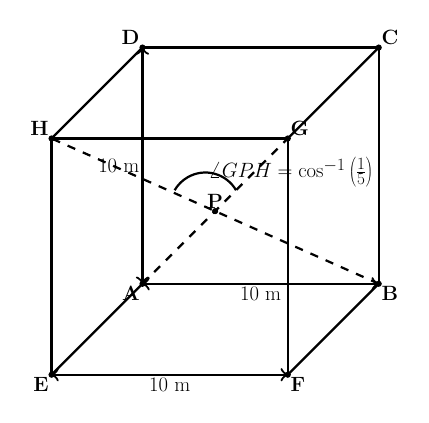
\begin{tikzpicture}[scale=0.3,transform shape]
    \coordinate (A) at (0, 0, 0);
    \coordinate (B) at (10, 0, 0);
    \coordinate (C) at (10, 10, 0);
    \coordinate (D) at (0, 10, 0);
    \coordinate (E) at (0, 0, 10);
    \coordinate (F) at (10, 0, 10);
    \coordinate (G) at (10, 10, 10);
    \coordinate (H) at (0, 10, 10);
    
    \coordinate (P) at (5, 5, 5); 

    \draw[thick] (A) -- (B) -- (C) -- (D) -- cycle;
    \draw[thick] (E) -- (F) -- (G) -- (H) -- cycle; 
    \draw[thick] (A) -- (E);
    \draw[thick] (B) -- (F);
    \draw[thick] (C) -- (G);
    \draw[thick] (D) -- (H);
    
    \draw[dashed, thick] (A) -- (G);
    \draw[dashed, thick] (B) -- (H);

    \foreach \point in {A, B, C, D, E, F, G, H, P} {
        \filldraw[black] (\point) circle (3pt);
    }

    \node at (A) [below left] {\Huge \textbf{A}};
    \node at (B) [below right] {\Huge \textbf{B}};
    \node at (C) [above right] {\Huge \textbf{C}};
    \node at (D) [above left] {\Huge \textbf{D}};
    \node at (E) [below left] {\Huge \textbf{E}};
    \node at (F) [below right] {\Huge \textbf{F}};
    \node at (G) [above right] {\Huge \textbf{G}};
    \node at (H) [above left] {\Huge \textbf{H}};
    \node at (P) [above] {\Huge \textbf{P}};

    \draw[<->, thick] (A) -- (B) node[midway, below] {\Huge 10 m};
    \draw[<->, thick] (A) -- (D) node[midway, left] {\Huge 10 m};
    \draw[<->, thick] (E) -- (F) node[midway, below] {\Huge 10 m};

    \draw[thick] (5.5, 5.5, 4) arc[start angle=30, end angle=150, radius=1.5] node[midway, right] {\Huge $\angle GPH = \cos^{-1}\left(\frac{1}{5}\right)$};

\end{tikzpicture}


\end{center}    
\begin{multicols}{4}
\begin{enumerate}
    \item $5$
    \item $2\sqrt{10}$
    \item $5\sqrt{3}$
    \item $5\sqrt{2}$
\end{enumerate}
\end{multicols}


%\end{enumerate}
%\end{document}



